% !TEX TS-program = pdflatexmk
\documentclass[12pt]{amsart}

%\usepackage[parfill]{parskip}    % Activate to begin paragraphs with an empty line rather than an indent

\usepackage[margin=1in]{geometry}

\usepackage{amsmath,amssymb,amsthm,latexsym,graphicx}
\usepackage[normalem]{ulem}
\usepackage{setspace} %used for doublespacing, etc.
\usepackage{hyperref}
\usepackage[dvipsnames,usenames]{color}
\usepackage{fancyhdr}
\pagestyle{fancy}
	\renewcommand{\headrulewidth}{0.5pt} % and the line
	\headsep=1cm
	
\DeclareGraphicsRule{.tif}{png}{.png}{`convert #1 `dirname #1`/`basename #1 .tif`.png}

%Some useful environments.
\newtheorem{theorem}{Theorem}
\newtheorem{corollary}[theorem]{Corollary}
\newtheorem{conjecture}[theorem]{Conjecture}
\newtheorem{lemma}[theorem]{Lemma}
\newtheorem{proposition}[theorem]{Proposition}
\newtheorem{definition}[theorem]{Definition}
\newtheorem{example}[theorem]{Example}
\newtheorem{axiom}{Axiom}
\theoremstyle{remark}
\newtheorem{remark}{Remark}
\newtheorem*{exercise}{Exercise}%[section]

%Some shortcuts helpful for our assignments
\newcommand{\bx}{\begin{exercise}}
\newcommand{\ex}{\end{exercise}}

%Some useful shortcuts for our favorite sets of numbers.
%Note, you can use these WITHOUT entering math mode
\def\RR{\ensuremath{\mathbb R}} 
\def\NN{\ensuremath{\mathbb N}}
\def\ZZ{\ensuremath{\mathbb Z}}
\def\QQ{{\ensuremath\mathbb Q}}
\def\CC{\ensuremath{\mathbb C}}
\def\EE{{\ensuremath\mathbb E}}

%Some useful shortcuts for formatting lists
\newcommand{\bc}{\begin{center}}
\newcommand{\ec}{\end{center}}
\newcommand{\be}{\begin{enumerate}}
\newcommand{\ee}{\end{enumerate}}
\newcommand{\bi}{\begin{itemize}}
\newcommand{\ei}{\end{itemize}}

%Some useful shortcuts for formatting mathematical symbols
\newcommand{\ol}[1]{\overline{#1}}
\newcommand{\oimp}[1]{\overset{#1}{\iff}} %labeled iff symbol
\newcommand{\bv}[1]{\ensuremath{ \vec{\mathbf{#1}}} } %makes a vector.
\newcommand{\mc}[1]{\ensuremath{\mathcal{#1}}} %put something in caligraphic font
\newcommand{\normale}{\trianglelefteq}
\newcommand{\normal}{\triangleleft}

%Code for formatting the proofs a little nicer for submitted homework
\makeatletter
\renewenvironment{proof}[1][\proofname]{\par\doublespacing
  \pushQED{\qed}%
  \normalfont \topsep6\p@\@plus6\p@\relax
  \list{}{%
    \settowidth{\leftmargin}{\itshape\proofname:\hskip\labelsep}%
    \setlength{\labelwidth}{0pt}%
    \setlength{\itemindent}{-\leftmargin}%
  }%
  \item[\hskip\labelsep\itshape#1\@addpunct{:}]\ignorespaces
}{%
  \popQED\endlist\@endpefalse
  \singlespacing
}
\makeatother


%Commenting tools for the professor
\newcommand{\mpg}[1]{\marginpar{ #1}} %to put comments in margins
\usepackage{soul}
\definecolor{highlight}{rgb}{1,0.6,0.6}
\sethlcolor{highlight}
\newcommand{\hlm}[1]{\colorbox{highlight}{$\displaystyle #1$}}
\newtheoremstyle{mycomment}{\topsep}{-0in}{\small \itshape \sffamily}{}{\small \itshape\sffamily}{:}{.5em}{}
\theoremstyle{mycomment}
\newtheorem*{acomment}{\color{BrickRed}{Comment}}
\newcommand{\com}[1]{{\color{OliveGreen}\begin{acomment}{#1} %#2 \color{black} 
\end{acomment}\noindent}}
\newcommand{\red}[1]{{\color{BrickRed} #1}}
\newcommand{\blue}[1]{{\color{MidnightBlue}#1}}
\newcommand{\green}[1]{{\color{OliveGreen}#1}}
\newcommand{\mwrong}[2]{\red{\cancel{#1}}\green{#2}}
\newcommand{\wrong}[2]{\red{\sout{#1}}\green{#2}}
\definecolor{OliveGreen}{rgb}{.3,.5,.2}
\definecolor{MidnightBlue}{rgb}{.3,.4,.6}
\newcommand{\pts}[1]{\hfill\blue{{#1}/5}}

\chead{MATH 371}
\pagestyle{fancy}
%Modify these items:
\rhead{\emph{Christopher Munoz}}
\lhead{\emph{HW 7}}

\begin{document}

\thispagestyle{fancy}
%§12.1 1, 3, 7, 9, 12.
\section*{Section 3.8} 



\begin{exercise}[3.121]Let $Y$ denote a random variable that has a Poisson distribution with mean $\lambda = 2$. Find:

\begin{enumerate}
    \item[(a)] $P(Y = 4)$
\begin{proof}[Solution]
	Poisson distribution function is $$P(Y=y)= \frac{e^{-\lambda} \lambda^y}{y!}$$
	$$P(Y=4) = \frac{e^{-2}(-2)^4}{4!} = 0.09022352$$
\end{proof}
    \item[(b)] $P(Y \geq 4)$
\begin{proof}[Solution]
	\begin{align*}
		P(Y \geq 4) &= 1 - [P(Y=3) + P(Y=2) + P(Y=1) + P(Y=0)] \\
			&= 1 - [\frac{e^{-2}(-2)^3}{3!} + \frac{e^{-2}(-2)^2}{2!} + \frac{e^{-2}(-2)^1}{1!} + \frac{e^{-2}(-2)^0}{0!}] \\
			&= 1 - [0.180447 + 0.2706706 + 0.2706706 + 0.1353353] \\
			&= 0.1428765
	\end{align*} 
	(table gives me 1-0.857 = 0.143 but wanted to do it full at least once)
\end{proof}
    \item[(c)] $P(Y < 4)$
\begin{proof}[Solution]
	\begin{align*}
		P(Y < 4) = P(Y \leq 3) = 0.857
	\end{align*}
	(table)
\end{proof}
    \item[(d)] $P(Y \geq 4 \mid Y \geq 2)$
\begin{proof}[Solution]
	\begin{align*}
		P(Y \geq 4 \mid Y \geq 2) = \frac{ P(Y \geq 4) \cap P(Y \geq 2)}{P(Y \geq 2)} = \frac{P(Y \geq 4)}{P(Y \geq 2)} = \frac{0.143}{1-0.406} = 0.241
	\end{align*}
	(table and prev prob)
\end{proof}
\end{enumerate} 
\end{exercise}
\begin{exercise}[3.122]
Customers arrive at a checkout counter in a department store according to a Poisson distribution at an average of seven per hour. During a given hour, what are the probabilities that:
 
\begin{enumerate}
    \item[(a)] no more than three customers arrive?
\begin{proof}[Solution]
	$$P(Y \leq 3) =  0.082$$
	(table)
\end{proof}
    \item[(b)] at least two customers arrive?
\begin{proof}[Solution]
	$$P(Y \geq 2) = 1 - P(Y \leq 1) = 1 - 0.007 = 0.993 $$
 
\end{proof}
    \item[(c)] exactly five customers arrive?
\begin{proof}[Solution]
	$$P(Y = 5) = \frac{e^{-7}7^5}{5!} = 0.1277167$$ 
\end{proof}
\end{enumerate} 
\end{exercise}

\begin{exercise}[3.125]
Refer to Exercise 3.122. If it takes approximately ten minutes to serve each customer, find the mean and variance of the total service time for customers arriving during a 1-hour period. (Assume that a sufficient number of servers are available so that no customer must wait for service.) Is it likely that the total service time will exceed 2.5 hours?

\begin{proof}[Solution]
	Note that $10$ minutes = $1/6$ of an hour, $E(Y) = \lambda$ and $V(Y) = \lambda$ for Poisson.
	\begin{align*}
		E(\frac{1}{6}Y) &= \frac{1}{6} E(Y) = \frac{1}{6} * 7 = 1.166667 \\
		V(\frac{1}{6}Y) &= (\frac{1}{6})^2V(Y) = \frac{1}{36} * 7 = 0.1944444 
	\end{align*}
	Not likely to exceed 2.5 hours of total service time since the variance is already so small, the standard deviation would be smaller
\end{proof}
\end{exercise}

\begin{exercise}[3.127]
The number of typing errors made by a typist has a Poisson distribution with an average of four errors per page. If more than four errors appear on a given page, the typist must retype the whole page. What is the probability that a randomly selected page does not need to be retyped?

\begin{proof}[Solution]
	$\lambda = 4$ and $Y \leq 4$ for this one.
	$$P(Y \leq 4) = 0.629$$ 
	(table)
\end{proof}
\end{exercise}

\begin{exercise}[3.131]
The number of knots in a particular type of wood has a Poisson distribution with an average of 1.5 knots in 10 cubic feet of the wood. Find the probability that a 10-cubic-foot block of the wood has at most 1 knot.

\begin{proof}[Solution]
	$\lambda = 1.5$ and $Y \leq 1$.
	$$P(Y \leq 1) = 0.558 $$
	(table really has everything doesn't it) 
\end{proof}
\end{exercise}

\begin{exercise}[3.134]
Consider a binomial experiment for $n = 20$, $p = .05$. Use Table 1, Appendix 3, to calculate the binomial probabilities for $Y = 0, 1, 2, 3$, and $4$. Calculate the same probabilities by using the Poisson approximation with $\lambda = np$. Compare.

\begin{proof}[Solution]
	Binomial Distribution for $P(Y \leq 4)$ for $n = 20$ and $p = 0.5$ is $0.997$ according to back table. For 
	our Poisson Distribution $\lambda = 20*0.05 = 1$, we refer to the table in the back and calculate it.
	\begin{align*}
		P(Y \leq 4) &= 0.996 \text{ (table)} \\
		P(Y \leq 4) &= P(Y = 0) + P(Y = 1) + P(Y = 2) + P(Y=3) + P(Y = 4) \\
			&= e^{-1}[\frac{1}{0!} + \frac{1}{1!} + \frac{1}{2!}+ \frac{1}{3!}+ \frac{1}{4!}] \\
			&= 0.9963402 \text{ (full calculation)}
	\end{align*}
	Depending on who you are, they are pretty close.
\end{proof}
\end{exercise}

\begin{exercise}[3.135]
A salesperson has found that the probability of a sale on a single contact is approximately .03. If the salesperson contacts 100 prospects, what is the approximate probability of making at least one sale?

\begin{proof}[Solution]
We use Poisson Approximation
	$$P(Y \geq 1) = 1 - P(Y = 0) = 1 - \frac{e^{-3} 3^0}{0!} = e^{-3} = 0.9502129$$
\end{proof}
\end{exercise}

\begin{exercise}[3.139]
In the daily production of a certain kind of rope, the number of defects per foot $Y$ is assumed to have a Poisson distribution with mean $\lambda = 2$. The profit per foot when the rope is sold is given by $X$, where $X = 50 - 2Y - Y^2$. Find the expected profit per foot.

\begin{proof}[Solution]
	\begin{align*}
		E(X) &= E[50 - 2Y - Y^2] \\
			&= E(50) - 2E(Y) - E(Y^2) \\
			&= 50 - 2(2) - [V(Y) + [E(Y)]^2] \\
			&= 50 - 4 - (2 + 4) \\ 
			&= 40
	\end{align*}
\end{proof}
\end{exercise}

\begin{exercise}[3.141]
A food manufacturer uses an extruder (a machine that produces bite-size cookies and snack food) that yields revenue for the firm at a rate of \$200 per hour when in operation. However, the extruder breaks down an average of two times every day it operates. If $Y$ denotes the number of breakdowns per day, the daily revenue generated by the machine is $R = 1600 - 50Y^2$. Find the expected daily revenue for the extruder.

\begin{proof}[Solution]
	\begin{align*}
		E(R) &= E[1600 - 50Y^2] \\
			&= E[1600] - 50E[Y^2] \\
			&= 1600 - 50[V(Y) + E(Y)^2] \\
			&= 1600 - 50[2 + 4] \\
			&= 1300
	\end{align*}
\end{proof}
\end{exercise}
\section*{Section 3.9}

\begin{exercise}[3.145]
If $Y$ has a binomial distribution with $n$ trials and probability of success $p$, show that the moment-generating function for $Y$ is
$$m(t) = (pe^t + q)^n, \text{ where } q = 1 - p.$$

\begin{proof}[Solution]
 The moment-generating function is $m(t) = E(e^{tY})$.
	
	For binomial distribution:
	\begin{align*}
		m(t) &= E(e^{tY}) = \sum_{y=0}^{n} e^{ty} \binom{n}{y} p^y q^{n-y} \\
		&= \sum_{y=0}^{n} \binom{n}{y} (pe^t)^y q^{n-y} \\
		&= (pe^t + q)^n \text{ by the binomial theorem}
	\end{align*}
\end{proof}
\end{exercise}

\begin{exercise}[3.146]
Differentiate the moment-generating function in Exercise 3.145 to find $E(Y)$ and $E(Y^2)$. Then find $V(Y)$.

\begin{proof}[Solution]
$m(t) = (pe^t + q)^n$.
	
	First derivative:
	$$m'(t) = n(pe^t + q)^{n-1} \cdot pe^t$$
	$$m'(0) = n(p + q)^{n-1} \cdot p = np = E(Y)$$
	
	Second derivative:
	$$m''(t) = n(n-1)(pe^t + q)^{n-2}(pe^t)^2 + n(pe^t + q)^{n-1}pe^t$$
	$$m''(0) = n(n-1)p^2 + np = E(Y^2)$$
	
	Therefore:
	\begin{align*}
		V(Y) &= E(Y^2) - [E(Y)]^2 \\
		&= n(n-1)p^2 + np - n^2p^2 \\
		&= n^2p^2 - np^2 + np - n^2p^2 \\
		&= np - np^2 = np(1-p) = npq
  \end{align*}
\end{proof}
\end{exercise}

\begin{exercise}[3.147]
If $Y$ has a geometric distribution with probability of success $p$, show that the moment-generating function for $Y$ is
$$m(t) = \frac{pe^t}{1 - qe^t}, \text{ where } q = 1 - p.$$

\begin{proof}[Solution]
 For geometric distribution, $P(Y = y) = pq^{y-1}$ for $y = 1, 2, 3, \ldots$
	
	\begin{align*}
		m(t) &= E(e^{tY}) = \sum_{y=1}^{\infty} e^{ty} pq^{y-1} \\
		&= pe^t \sum_{y=1}^{\infty} (qe^t)^{y-1} \\
		&= pe^t \sum_{k=0}^{\infty} (qe^t)^k \text{ (let } k = y-1) \\
		&= pe^t \cdot \frac{1}{1 - qe^t} \text{ (geometric series, } |qe^t| < 1) \\
		&= \frac{pe^t}{1 - qe^t}
	\end{align*}
\end{proof}
\end{exercise}

\begin{exercise}[3.149]
Refer to Exercise 3.145. Use the uniqueness of moment-generating functions to give the distribution of a random variable with moment-generating function $m(t) = (0.6e^t + 0.4)^3$.

\begin{proof}[Solution]
 Comparing $m(t) = (0.6e^t + 0.4)^3$ with the binomial MGF $m(t) = (pe^t + q)^n$:
	
	We have $p = 0.6$, $q = 0.4$, and $n = 3$.
	
	Therefore, $Y$ has a \textbf{binomial distribution with $n = 3$ and $p = 0.6$}.
\end{proof}
\end{exercise}

\begin{exercise}[3.151]
Refer to Exercise 3.145. If $Y$ has moment-generating function $m(t) = (0.7e^t + 0.3)^{10}$, what is $P(Y \leq 5)$?

\begin{proof}[Solution]
 From the MGF, $Y$ has a binomial distribution with $n = 10$ and $p = 0.7$.
	
	Using Table 1 (Binomial table) with $n = 10$ and $p = 0.7$:
	$$P(Y \leq 5) = 0.150$$
\end{proof}
\end{exercise}

\begin{exercise}[3.153]
Find the distributions of the random variables that have each of the following moment-generating functions:

\begin{enumerate}
    \item[(a)] $m(t) = [(1/3)e^t + (2/3)]^5$
\begin{proof}[Solution]
 This is a binomial MGF with $p = 1/3$, $q = 2/3$, and $n = 5$.
	
	Therefore, $Y \sim \text{Binomial}(n = 5, p = 1/3)$.
\end{proof}
    \item[(b)] $m(t) = \frac{e^t}{2 - e^t}$
\begin{proof}[Solution]
 Rewrite: $m(t) = \frac{e^t}{2 - e^t} = \frac{(1/2)e^t}{1 - (1/2)e^t}$
	
	This matches the geometric MGF with $p = 1/2$ and $q = 1/2$.
	
	Therefore, $Y \sim \text{Geometric}(p = 1/2)$.
\end{proof}
    \item[(c)] $m(t) = e^{2(e^t - 1)}$
\begin{proof}[Solution]
 The Poisson MGF is $m(t) = e^{\lambda(e^t - 1)}$.
	
	Comparing with $m(t) = e^{2(e^t - 1)}$, we have $\lambda = 2$.
	
	Therefore, $Y \sim \text{Poisson}(\lambda = 2)$.
\end{proof}
\end{enumerate} 
\end{exercise}

\begin{exercise}[3.155]
Let $m(t) = \frac{1}{6}e^t + \frac{2}{6}e^{2t} + \frac{3}{6}e^{3t}$. Find the following:

\begin{enumerate}
    \item[(a)] $E(Y)$
\begin{proof}[Solution]
 $m'(t) = \frac{1}{6}e^t + \frac{4}{6}e^{2t} + \frac{9}{6}e^{3t}$
	
	$E(Y) = m'(0) = \frac{1}{6} + \frac{4}{6} + \frac{9}{6} = \frac{14}{6} = \frac{7}{3}$
\end{proof}
    \item[(b)] $V(Y)$
\begin{proof}[Solution]
 $m''(t) = \frac{1}{6}e^t + \frac{8}{6}e^{2t} + \frac{27}{6}e^{3t}$
	
	$E(Y^2) = m''(0) = \frac{1}{6} + \frac{8}{6} + \frac{27}{6} = \frac{36}{6} = 6$
	
	$V(Y) = E(Y^2) - [E(Y)]^2 = 6 - \left(\frac{7}{3}\right)^2 = 6 - \frac{49}{9} = \frac{54 - 49}{9} = \frac{5}{9}$
\end{proof}
    \item[(c)] The distribution of $Y$
\begin{proof}[Solution]
 The MGF has the form $m(t) = \sum p(y) e^{yt}$.
	
	Comparing: $p(1) = 1/6$, $p(2) = 2/6 = 1/3$, $p(3) = 3/6 = 1/2$
	
	Therefore, $Y$ is a discrete random variable with probability function:
	$$p(y) = \begin{cases}
	1/6, & y = 1 \\
	1/3, & y = 2 \\
	1/2, & y = 3 \\
	0, & \text{otherwise}
	\end{cases}$$
\end{proof}
\end{enumerate} 
\end{exercise}

\section*{Section 3.11}

\begin{exercise}[3.167]
Let $Y$ be a random variable with mean 11 and variance 9. Using Tchebysheff's theorem, find:

\begin{enumerate}
    \item[(a)] a lower bound for $P(6 < Y < 16)$
\begin{proof}[Solution]
 $\mu = 11$, $\sigma^2 = 9$, so $\sigma = 3$.
	
	The interval $(6, 16)$ is $\mu \pm 5 = 11 \pm 5$.
	
	So $k = 5/3$ standard deviations.
	
	By Tchebysheff's theorem:
	$$P(|Y - \mu| < k\sigma) \geq 1 - \frac{1}{k^2} = 1 - \frac{1}{(5/3)^2} = 1 - \frac{9}{25} = \frac{16}{25} = 0.64$$
\end{proof}
    \item[(b)] the value of $C$ such that $P(|Y - 11| \geq C) \leq 0.09$
\begin{proof}[Solution]
 By Tchebysheff's theorem: $P(|Y - \mu| \geq k\sigma) \leq \frac{1}{k^2}$
	
	We want $\frac{1}{k^2} = 0.09$, so $k^2 = \frac{1}{0.09} = \frac{100}{9}$, thus $k = \frac{10}{3}$.
	
	Therefore:
	$$C = k\sigma = \frac{10}{3} \cdot 3 = 10$$
\end{proof}
\end{enumerate} 
\end{exercise}

\begin{exercise}[3.168]
Would you rather take a multiple-choice test or a full-recall test? If you have absolutely no knowledge of the test material, you will score zero on a full-recall test. However, if you are given 5 choices for each multiple-choice question, you have at least one chance in five of guessing each correct answer! Suppose that a multiple-choice exam contains 100 questions, each with 5 possible answers, and you guess the answer to each of the questions.

\begin{enumerate}
    \item[(a)] What is the expected value of the number $Y$ of questions that will be correctly answered?
\begin{proof}[Solution]
 $Y \sim \text{Binomial}(n = 100, p = 1/5 = 0.2)$
	
	$E(Y) = np = 100(0.2) = 20$
\end{proof}
    \item[(b)] Find the standard deviation of $Y$.
\begin{proof}[Solution]
 $V(Y) = npq = 100(0.2)(0.8) = 16$
	
	$\sigma = \sqrt{16} = 4$
\end{proof}
    \item[(c)] Calculate the intervals $\mu \pm 2\sigma$ and $\mu \pm 3\sigma$.
\begin{proof}[Solution]
 $\mu \pm 2\sigma = 20 \pm 2(4) = 20 \pm 8 = (12, 28)$
	
	$\mu \pm 3\sigma = 20 \pm 3(4) = 20 \pm 12 = (8, 32)$
\end{proof}
    \item[(d)] If the results of the exam are curved so that 50 correct answers is a passing score, are you likely to receive a passing score? Explain.
\begin{proof}[Solution]
 50 is $\frac{50 - 20}{4} = 7.5$ standard deviations above the mean.
	
	By Tchebysheff's theorem, $P(|Y - 20| \geq 30) \leq \frac{1}{(7.5)^2} = \frac{1}{56.25} \approx 0.018$.
	
	Therefore, it is \textbf{very unlikely} to receive a passing score (probability less than 2\%).
\end{proof}
\end{enumerate} 
\end{exercise}

\begin{exercise}[3.171]
For a certain type of soil the number of wireworms per cubic foot has a mean of 100. Assuming a Poisson distribution of wireworms, give an interval that will include at least $5/9$ of the sample values of wireworm counts obtained from a large number of 1-cubic-foot samples.

\begin{proof}[Solution]
 For Poisson: $\mu = \lambda = 100$ and $\sigma^2 = \lambda = 100$, so $\sigma = 10$.
	
	By Tchebysheff's theorem: $P(|Y - \mu| < k\sigma) \geq 1 - \frac{1}{k^2}$
	
	We want $1 - \frac{1}{k^2} = \frac{5}{9}$, so $\frac{1}{k^2} = \frac{4}{9}$, thus $k^2 = \frac{9}{4}$ and $k = \frac{3}{2}$.
	
	The interval is:
	$$\mu \pm k\sigma = 100 \pm \frac{3}{2}(10) = 100 \pm 15 = (85, 115)$$
\end{proof}
\end{exercise}

\section*{4.2}
\begin{exercise}[4.1]
Let $Y$ be a random variable with $p(y)$ given in the table below.
\begin{center}
\begin{tabular}{c|cccc}
$y$ & 1 & 2 & 3 & 4 \\
\hline
$p(y)$ & .4 & .3 & .2 & .1
\end{tabular}
\end{center}

\begin{enumerate}
    \item[(a)] Give the distribution function, $F(y)$. Be sure to specify the value of $F(y)$ for all $y$, $-\infty < y < \infty$.
\begin{proof}[Solution]
 $$F(y) = P(Y \leq y) = \begin{cases}
	0, & y < 1 \\
	0.4, & 1 \leq y < 2 \\
	0.7, & 2 \leq y < 3 \\
	0.9, & 3 \leq y < 4 \\
	1, & y \geq 4
	\end{cases}$$
\end{proof}
    \item[(b)] Sketch the distribution function given in part (a).
\begin{proof}[Solution]
 	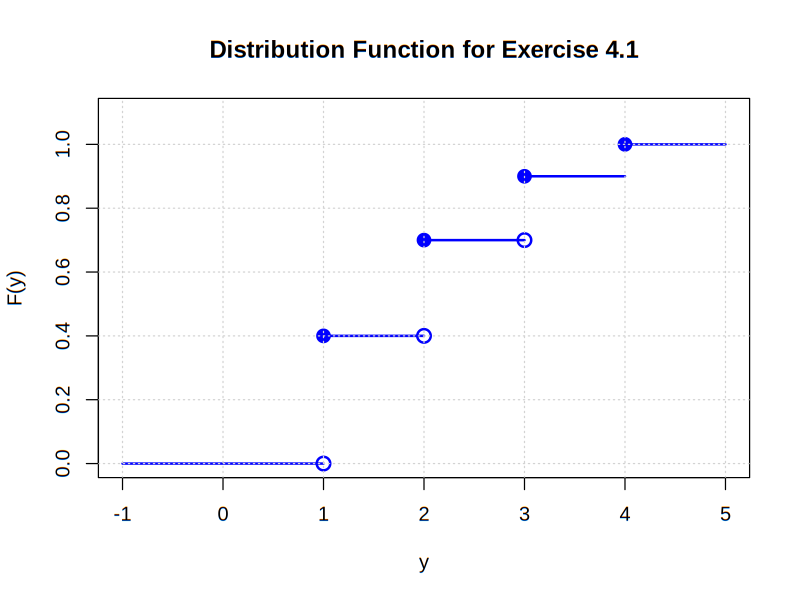
\includegraphics[width=0.7\textwidth]{exercise_4_1b.png}
\end{proof}
\end{enumerate} 
\end{exercise}

\begin{exercise}[4.3]
A Bernoulli random variable is one that assumes only two values, 0 and 1 with $p(1) = p$ and $p(0) = 1 - p \equiv q$.

\begin{enumerate}
    \item[(a)] Sketch the corresponding distribution function.
\begin{proof}[Solution]
 	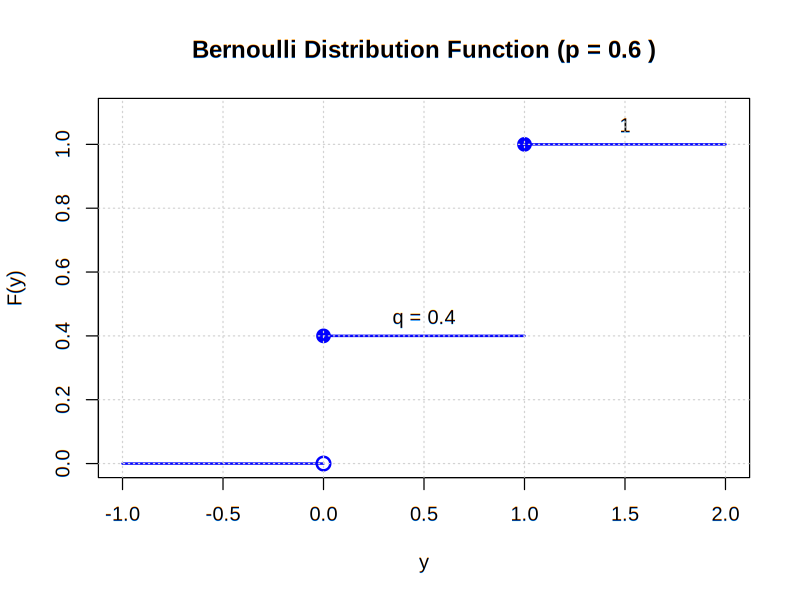
\includegraphics[width=0.7\textwidth]{exercise_4_3a.png}
\end{proof}
    \item[(b)] Show that this distribution function has the properties given in Theorem 4.1.
\begin{proof}[Solution]
 Theorem 4.1 properties:
	\begin{enumerate}
		\item $F(-\infty) = 0$: Yes, $\lim_{y \to -\infty} F(y) = 0$ 
		\item $F(\infty) = 1$: Yes, $\lim_{y \to \infty} F(y) = 1$ 
		\item $F$ is non-decreasing: $0 \leq q \leq 1$ since $q = 1-p$ and $0 \leq p \leq 1$ 
		\item $F$ is right-continuous: At each point, $F$ equals its right-hand limit 
	\end{enumerate}
\end{proof}
\end{enumerate} 
\end{exercise}

\begin{exercise}[4.5]
Suppose that $Y$ is a random variable that takes on only integer values $1, 2, \ldots$ and has distribution function $F(y)$. Show that the probability function $p(y) = P(Y = y)$ is given by
$$p(y) = \begin{cases}
F(1), & y = 1, \\
F(y) - F(y-1), & y = 2, 3, \ldots
\end{cases}$$

\begin{proof}[Solution]
 For $y = 1$: $P(Y = 1) = P(Y \leq 1) = F(1)$ since $Y$ takes integer values $\geq 1$.
	
	For $y \geq 2$:
	\begin{align*}
		P(Y = y) &= P(Y \leq y) - P(Y \leq y-1) \\
		&= F(y) - F(y-1)
  \end{align*}
\end{proof}
\end{exercise}

\begin{exercise}[4.7]
Let $Y$ be a binomial random variable with $n = 10$ and $p = 0.2$.

\begin{enumerate}
    \item[(a)] Use Table 1, Appendix 3, to obtain $P(2 < Y < 5)$ and $P(2 \leq Y < 5)$. Are the probabilities that $Y$ falls in the intervals $(2, 5)$ and $[2, 5)$ equal? Why or why not?
\begin{proof}[Solution]
 $P(2 < Y < 5) = P(Y = 3) + P(Y = 4) = P(Y \leq 4) - P(Y \leq 2) = 0.967 - 0.678 = 0.289$
	
	$P(2 \leq Y < 5) = P(Y = 2) + P(Y = 3) + P(Y = 4) = P(Y \leq 4) - P(Y \leq 1) = 0.967 - 0.376 = 0.591$
	
	not equal because $Y$ is discrete. For discrete variables, $(2,5)$ excludes 2 while $[2,5)$ includes 2.
\end{proof}
    \item[(b)] Use Table 1, Appendix 3, to obtain $P(2 < Y \leq 5)$ and $P(2 \leq Y \leq 5)$. Are these two probabilities equal? Why or why not?
\begin{proof}[Solution]
 $P(2 < Y \leq 5) = P(Y = 3) + P(Y = 4) + P(Y = 5) = P(Y \leq 5) - P(Y \leq 2) = 0.994 - 0.678 = 0.316$
	
	$P(2 \leq Y \leq 5) = P(Y \leq 5) - P(Y \leq 1) = 0.994 - 0.376 = 0.618$
	
	not equal because including/excluding $Y = 2$ makes a difference for discrete variables.
\end{proof}
    \item[(c)] Earlier in this section, we argued that if $Y$ is continuous and $a < b$, then $P(a < Y < b) = P(a \leq Y < b)$. Does the result in part (a) contradict this claim? Why?
\begin{proof}[Solution]
 no this does not contradict the claim. The claim is specifically for continuous random variables, where $P(Y = a) = 0$ for any specific value $a$. Here, $Y$ is \textbf{discrete}, so $P(Y = 2) \neq 0$, and therefore the inclusion/exclusion of endpoints matters.
\end{proof}
\end{enumerate} 
\end{exercise}

\begin{exercise}[4.9]
A random variable $Y$ has the following distribution function:
$$F(y) = P(Y \leq y) = \begin{cases}
0, & \text{for } y < 2, \\
1/8, & \text{for } 2 \leq y < 2.5, \\
3/16, & \text{for } 2.5 \leq y < 4, \\
1/2, & \text{for } 4 \leq y < 5.5, \\
5/8, & \text{for } 5.5 \leq y < 6, \\
11/16, & \text{for } 6 \leq y < 7, \\
1, & \text{for } y \geq 7.
\end{cases}$$

\begin{enumerate}
    \item[(a)] Is $Y$ a continuous or discrete random variable? Why?
\begin{proof}[Solution]
 
\end{proof}
    \item[(b)] What values of $Y$ are assigned positive probabilities?
\begin{proof}[Solution]
 
\end{proof}
    \item[(c)] Find the probability function for $Y$.
\begin{proof}[Solution]
 
\end{proof}
    \item[(d)] What is the median, $\phi_{.5}$, of $Y$?
\begin{proof}[Solution]
 
\end{proof}
\end{enumerate} 
\end{exercise}

\begin{exercise}[4.11]
Suppose that $Y$ possesses the density function
$$f(y) = \begin{cases}
cy, & 0 \leq y \leq 2, \\
0, & \text{elsewhere}.
\end{cases}$$

\begin{enumerate}
    \item[(a)] Find the value of $c$ that makes $f(y)$ a probability density function.
\begin{proof}[Solution]
 For $f(y)$ to be a pdf: $\int_{-\infty}^{\infty} f(y) dy = 1$
	
	$$\int_0^2 cy \, dy = c \left[\frac{y^2}{2}\right]_0^2 = c \cdot 2 = 1$$
	
	Therefore, $c = 1/2$.
\end{proof}
    \item[(b)] Find $F(y)$.
\begin{proof}[Solution]
 For $y < 0$: $F(y) = 0$
	
	For $0 \leq y \leq 2$:
	$$F(y) = \int_0^y \frac{1}{2}t \, dt = \frac{1}{2} \cdot \frac{y^2}{2} = \frac{y^2}{4}$$
	
	For $y > 2$: $F(y) = 1$
	
	$$F(y) = \begin{cases}
	0, & y < 0 \\
	y^2/4, & 0 \leq y \leq 2 \\
	1, & y > 2
	\end{cases}$$
\end{proof}
    \item[(c)] Graph $f(y)$ and $F(y)$.
\begin{proof}[Solution]
 	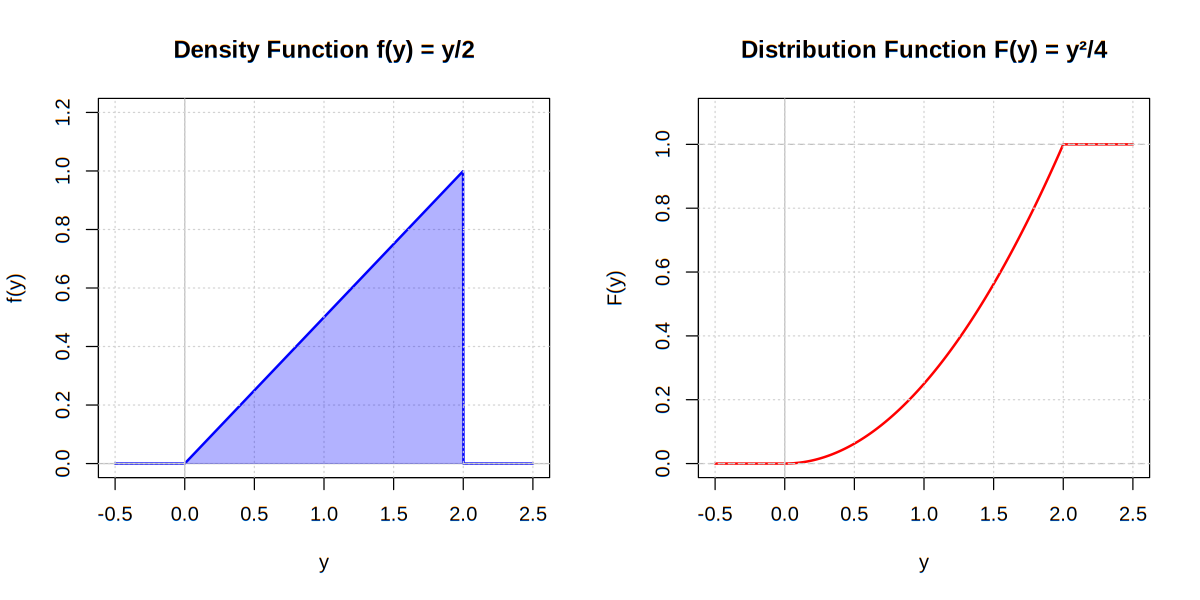
\includegraphics[width=0.7\textwidth]{exercise_4_11c.png}
\end{proof}
    \item[(d)] Use $F(y)$ to find $P(1 \leq Y \leq 2)$.
\begin{proof}[Solution]
 $$P(1 \leq Y \leq 2) = F(2) - F(1) = 1 - \frac{1}{4} = \frac{3}{4}$$
\end{proof}
    \item[(e)] Use $f(y)$ and geometry to find $P(1 \leq Y \leq 2)$.
\begin{proof}[Solution]
 	$$P(1 \leq Y \leq 2) = \int_1^2 \frac{y}{2} dy = \frac{1}{2} \left[\frac{y^2}{2}\right]_1^2 = \frac{1}{4}(4 - 1) = \frac{3}{4}$$
	
	Geometrically, this is the area of a trapezoid with parallel sides $f(1) = 1/2$ and $f(2) = 1$, and height 1:
	$$\text{Area} = \frac{1}{2}(1/2 + 1)(1) = \frac{3}{4}$$
\end{proof}
\end{enumerate} 
\end{exercise}

\begin{exercise}[4.13]
A supplier of kerosene has a 150-gallon tank that is filled at the beginning of each week. His weekly demand shows a relative frequency behavior that increases steadily up to 100 gallons and then levels off between 100 and 150 gallons. If $Y$ denotes weekly demand in hundreds of gallons, the relative frequency of demand can be modeled by
$$f(y) = \begin{cases}
y, & 0 \leq y \leq 1, \\
1, & 1 < y \leq 1.5, \\
0, & \text{elsewhere}.
\end{cases}$$

\begin{enumerate}
    \item[(a)] Find $F(y)$.
\begin{proof}[Solution]
 For $y < 0$: $F(y) = 0$
	
	For $0 \leq y \leq 1$: $F(y) = \int_0^y t \, dt = \frac{y^2}{2}$
	
	For $1 < y \leq 1.5$: $F(y) = \int_0^1 t \, dt + \int_1^y 1 \, dt = \frac{1}{2} + (y - 1) = y - \frac{1}{2}$
  For $y > 1.5$: $F(y) = 1$
  \begin{align*}
	F(y) = \begin{cases}
	0, & y < 0 \\
	y^2/2, & 0 \leq y \leq 1 \\
	y - 1/2, & 1 < y \leq 1.5 \\
	1, & y > 1.5
	\end{cases}
\end{align*}
\end{proof}
    \item[(b)] Find $P(0 \leq Y \leq 0.5)$.
\begin{proof}[Solution]
 	$$P(0 \leq Y \leq 0.5) = F(0.5) - F(0) = \frac{(0.5)^2}{2} - 0 = \frac{0.25}{2} = 0.125$$
\end{proof}
    \item[(c)] Find $P(0.5 \leq Y \leq 1.2)$.
\begin{proof}[Solution]
 	$$P(0.5 \leq Y \leq 1.2) = F(1.2) - F(0.5) = \left(1.2 - \frac{1}{2}\right) - \frac{(0.5)^2}{2} = 0.7 - 0.125 = 0.575$$
\end{proof}
\end{enumerate} 
\end{exercise}

\begin{exercise}[4.17]
The length of time required by students to complete a one-hour exam is a random variable with a density function given by
$$f(y) = \begin{cases}
cy^2 + y, & 0 \leq y \leq 1, \\
0, & \text{elsewhere}.
\end{cases}$$

\begin{enumerate}
    \item[(a)] Find $c$.
\begin{proof}[Solution]
 	For $f(y)$ to be a pdf: $\int_{-\infty}^{\infty} f(y) dy = 1$
	
	$$\int_0^1 (cy^2 + y) dy = \left[\frac{cy^3}{3} + \frac{y^2}{2}\right]_0^1 = \frac{c}{3} + \frac{1}{2} = 1$$
	
	$$\frac{c}{3} = \frac{1}{2} \implies c = \frac{3}{2}$$
\end{proof}
    \item[(b)] Find $F(y)$.
\begin{proof}[Solution]
For $y < 0$: $F(y) = 0$
	
	For $0 \leq y \leq 1$:
	$$F(y) = \int_0^y \left(\frac{3}{2}t^2 + t\right) dt = \left[\frac{t^3}{2} + \frac{t^2}{2}\right]_0^y = \frac{y^3}{2} + \frac{y^2}{2} = \frac{y^2(y+1)}{2}$$
	
	For $y > 1$: $F(y) = 1$
	
	$$F(y) = \begin{cases}
	0, & y < 0 \\
	\frac{y^2(y+1)}{2}, & 0 \leq y \leq 1 \\
	1, & y > 1
	\end{cases}$$
\end{proof}
    \item[(c)] Graph $f(y)$ and $F(y)$.
\begin{proof}[Solution]
 	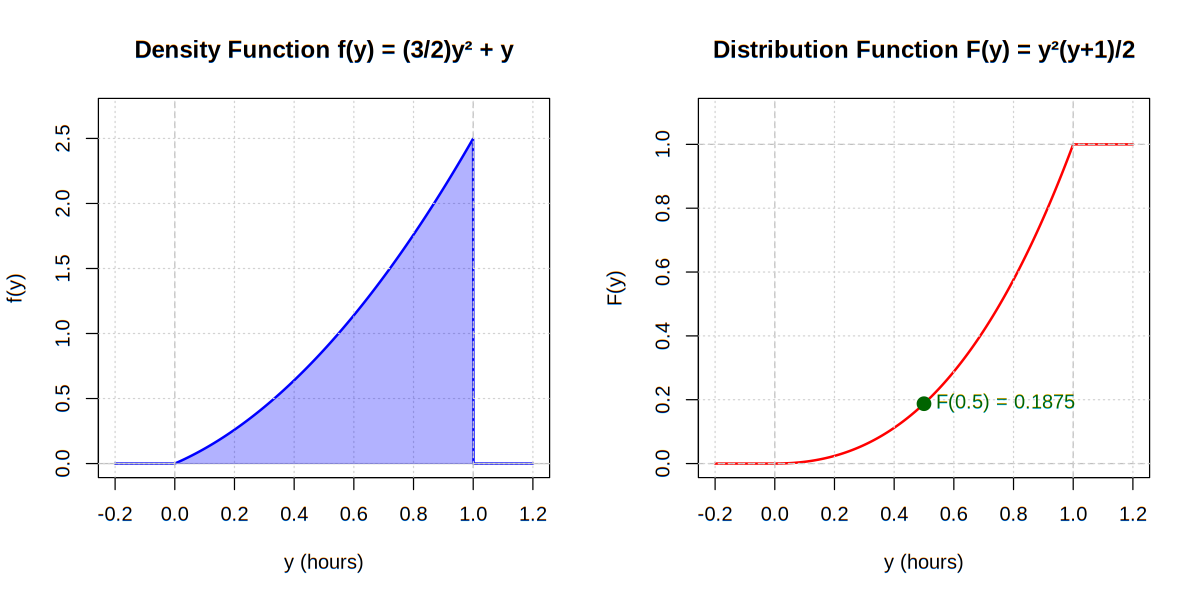
\includegraphics[width=0.7\textwidth]{exercise_4_17c.png}
\end{proof}
    \item[(d)] Use $F(y)$ in part (b) to find $F(-1)$, $F(0)$, and $F(1)$.
\begin{proof}[Solution]
 	$$F(-1) = 0$$
	$$F(0) = 0$$
	$$F(1) = \frac{1^2(1+1)}{2} = 1$$
\end{proof}
    \item[(e)] Find the probability that a randomly selected student will finish in less than half an hour.
\begin{proof}[Solution]
 	$$P(Y < 0.5) = F(0.5) = \frac{(0.5)^2(0.5+1)}{2} = \frac{0.25 \cdot 1.5}{2} = \frac{0.375}{2} = 0.1875$$
\end{proof}
    \item[(f)] Given that a particular student needs at least 15 minutes to complete the exam, find the probability that she will require at least 30 minutes to finish.
\begin{proof}[Solution]
 15 minutes = 0.25 hours, 30 minutes = 0.5 hours
	
	$$P(Y \geq 0.5 | Y \geq 0.25) = \frac{P(Y \geq 0.5)}{P(Y \geq 0.25)} = \frac{1 - F(0.5)}{1 - F(0.25)}$$
	
	$$F(0.25) = \frac{(0.25)^2(1.25)}{2} = \frac{0.078125}{2} = 0.0390625$$
	
	$$P(Y \geq 0.5 | Y \geq 0.25) = \frac{1 - 0.1875}{1 - 0.0390625} = \frac{0.8125}{0.9609375} \approx 0.846$$
\end{proof}
\end{enumerate} 
\end{exercise}

\begin{exercise}[4.19]
Let the distribution function of a random variable $Y$ be
$$F(y) = \begin{cases}
0, & y \leq 0, \\
\frac{y}{8}, & 0 < y < 2, \\
\frac{y^2}{16}, & 2 \leq y < 4, \\
1, & y \geq 4.
\end{cases}$$

\begin{enumerate}
    \item[(a)] Find the density function of $Y$.
\begin{proof}[Solution]
	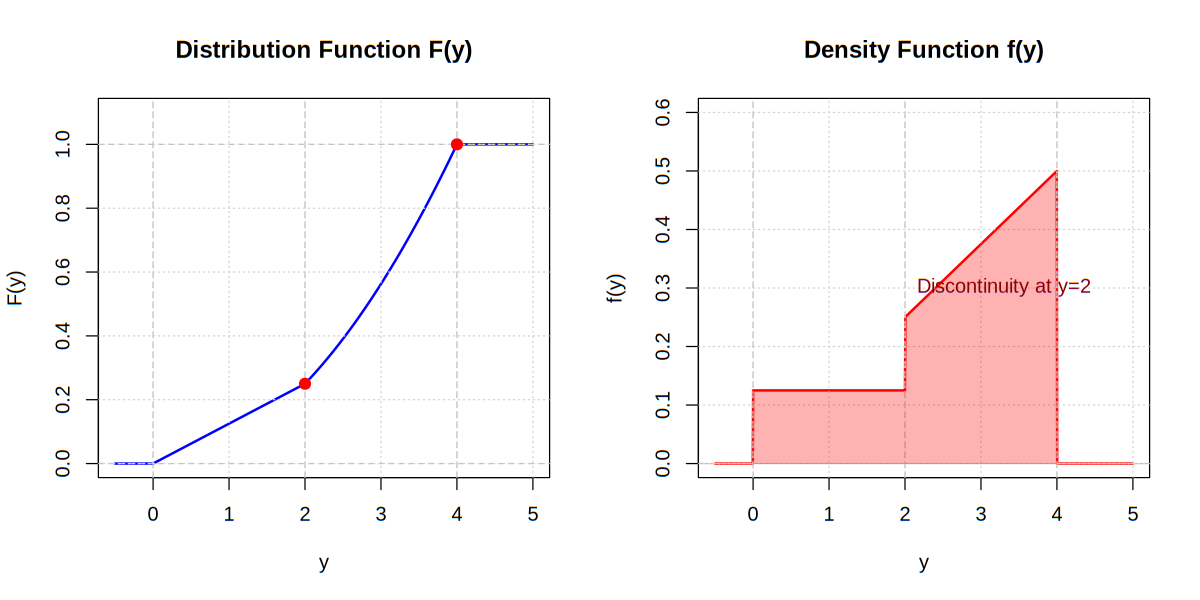
\includegraphics[width=0.7\textwidth]{exercise_4_19.png}
  	Note: At $y = 2$, $F$ is not differentiable (there's a corner), so the density is undefined there.
\end{proof}
    \item[(b)] Find $P(1 \leq Y \leq 3)$.
\begin{proof}[Solution]
 	$$P(1 \leq Y \leq 3) = F(3) - F(1) = \frac{9}{16} - \frac{1}{8} = \frac{9}{16} - \frac{2}{16} = \frac{7}{16}$$
\end{proof}
    \item[(c)] Find $P(Y \geq 1.5)$.
\begin{proof}[Solution]
 	$$P(Y \geq 1.5) = 1 - F(1.5) = 1 - \frac{1.5}{8} = 1 - \frac{3}{16} = \frac{13}{16}$$
\end{proof}
    \item[(d)] Find $P(Y \geq 1 \mid Y \leq 3)$.
\begin{proof}[Solution]
 	$$P(Y \geq 1 | Y \leq 3) = \frac{P(1 \leq Y \leq 3)}{P(Y \leq 3)} = \frac{F(3) - F(1)}{F(3)} = \frac{9/16 - 1/8}{9/16} = \frac{7/16}{9/16} = \frac{7}{9}$$
\end{proof}
\end{enumerate} 
\end{exercise}

 \end{document} 
